\documentclass[conference]{IEEEtran}
\IEEEoverridecommandlockouts
\usepackage{cite}
\usepackage{amsmath,amssymb,amsfonts}
\usepackage{algorithm}
\usepackage{algorithmic}
\usepackage{graphicx}
\usepackage{textcomp}
\usepackage{xcolor}
\usepackage{url}
\usepackage{listings}
\usepackage{booktabs}
\usepackage{multirow}

\lstset{
  language=Python,
  basicstyle=\scriptsize\ttfamily,
  breaklines=true,
  columns=fullflexible,
  keepspaces=true,
  showstringspaces=false,
  numbers=left,
  numberstyle=\tiny,
  xleftmargin=1.6em,
  framexleftmargin=1.2em,
  aboveskip=0.4\baselineskip,
  belowskip=0.4\baselineskip,
}

\def\BibTeX{{\rm B\kern-.05em{\sc i\kern-.025em b}\kern-.08em
    T\kern-.1667em\lower.7ex\hbox{E}\kern-.125emX}}
\begin{document}

\title{Comparing Niching Methods for Multimodal Function Optimization:\\
Deterministic Crowding versus Fitness Sharing}

% \author{\IEEEauthorblockN{Cong Hoan Nguyen}
% \IEEEauthorblockA{{Computer Science & Engineering Department} \\
% {University of Louisville} \\
% {Louisville, KY, USA} \\
% {c0nguy10@louisville.edu}}
% \and
% \IEEEauthorblockN{Anesa Hozdic}
% \IEEEauthorblockA{{Computer Science & Engineering Department} \\
% {University of Louisville} \\
% {Louisville, KY, USA} \\
% {anesa.hozdic@louisville.edu}}
% }

\author{\IEEEauthorblockN{1\textsuperscript{st} Cong Hoan Nguyen}
\IEEEauthorblockA{\textit{CSE Department} \\
\textit{University of Louisville}\\
Louisville, KY, USA \\
c0nguy10@louisville.edu}
\and
\IEEEauthorblockN{2\textsuperscript{nd} Anesa Hozdic}
\IEEEauthorblockA{\textit{CSE Department} \\
\textit{University of Louisville}\\
Louisville, KY, USA \\
anesa.hozdic@louisville.edu}

}

\maketitle

\begin{abstract}
Genetic algorithms (GAs) are designed to converge to a single optimum, yet many
problems require locating every optimum of a multimodal landscape. This project
compares two niching methods---deterministic crowding and fitness
sharing---against a standard GA on the benchmark functions M1 and M4. All three
algorithms share the same 10-bit binary encoding, two-point crossover, and
bit-flip mutation operators; they differ only in how parents are selected and
how offspring are inserted. We sweep two crossover rates ($P_c = 0.60, 0.95$)
and two mutation rates ($P_m = 0.01, 0.10$) and average every metric over 10
independent runs per configuration (240 runs total, 300 generations each).
Deterministic crowding found all five peaks of M1 in every run
($5.0 \pm 0.00$) but lost the shorter peaks of the unequal-height function M4
($1.9$--$2.3$ of 5). Fitness sharing was the most robust method overall on M4
($3.5$--$3.9$ of 5) and remained strong on M1 ($3.8$--$4.2$). The standard GA
rarely exceeded $3.2$ peaks and collapsed toward a single peak at low mutation
rates. The results illustrate that the best niching method depends on the
relative heights of the peaks, and that best fitness alone hides diversity
collapse.
\end{abstract}

\begin{IEEEkeywords}
genetic algorithms, niching methods, multimodal optimization, fitness sharing,
deterministic crowding
\end{IEEEkeywords}

\section{Introduction}
\label{sec:intro}

Many real-world optimization problems are multimodal: several solutions are
acceptable, and in some cases \emph{all} of the near-optimal solutions are
wanted rather than a single global best. A standard genetic algorithm (GA)
\cite{b1} uses fitness-proportionate selection, which concentrates the
population on whichever peak currently holds the highest-fitness individual;
genetic drift then removes individuals from the other peaks and the population
collapses onto one mode. Niching methods \cite{b2,b3} extend the GA so that
several subpopulations (niches) can be maintained at different optima at the
same time.

The objective of this project is to implement and comparatively evaluate two
classic niching methods---\emph{deterministic crowding} \cite{b2} and
\emph{fitness sharing} \cite{b3}---against an unmodified (standard) GA on the
two one-dimensional benchmark functions M1 and M4 defined for this assignment:

\begin{equation}
\mathrm{M1}(x) = \sin^{6}(5\pi x), \qquad x \in [0,1],
\label{eq:m1}
\end{equation}
\begin{multline}
\mathrm{M4}(x) = e^{-2(\ln 2)\left(\frac{x-0.08}{0.854}\right)^{2}}\\
\cdot \sin^{6}\!\left(5\pi\left[x^{0.75}-0.05\right]\right), \qquad x \in [0,1].
\label{eq:m4}
\end{multline}

Both functions have five peaks on $[0,1]$, but they differ in a way that turns
out to be decisive. M1 has five \emph{equal-height} peaks
($\mathrm{M1}=1$ at $x = 0.1, 0.3, 0.5, 0.7, 0.9$), whereas the Gaussian
envelope in M4 makes its five peaks \emph{unequal in height}
($\approx 1.000, 0.947, 0.771, 0.504, 0.252$ at
$x \approx 0.08, 0.245, 0.45, 0.68, 0.93$).

The experimental questions addressed in this report are: (i) how much does
each niching method improve peak discovery over a standard GA; (ii) how do the
crossover rate $P_c$ and mutation rate $P_m$ affect each method; and (iii)
does the ranking of the methods change between the equal-height (M1) and
unequal-height (M4) landscapes? We answer them with a full factorial protocol:
2 functions $\times$ 3 methods $\times$ 2 values of $P_c$ $\times$ 2 values of
$P_m$ $\times$ 10 seeds $= 240$ runs of 300 generations each, reporting
averages over the 10 runs for every configuration.

Section~\ref{sec:methods} describes the algorithms in pseudocode and equations
and summarizes the implementation. Section~\ref{sec:protocol} specifies the
experimental protocol. Section~\ref{sec:results} tabulates and plots the
results, Section~\ref{sec:analysis} analyzes them, and
Section~\ref{sec:conclusions} concludes. Source code, additional figures, and
the video link are in the Appendix.

\section{Methods}
\label{sec:methods}

\subsection{Common GA skeleton}
\label{sec:skeleton}

All three algorithms share the same representation and genetic operators. An
individual is a 10-bit binary string $\mathbf{b} = (b_1,\ldots,b_{10})$
decoded to the phenotype
\begin{equation}
x(\mathbf{b}) = \sum_{i=1}^{10} b_i \, 2^{-i} \in [0,1),
\label{eq:decode}
\end{equation}
which gives a search resolution of $2^{-10} \approx 0.00098$. Fitness is the
raw objective value, $f(\mathbf{b}) = \mathrm{M}(x(\mathbf{b}))$.
Parents are chosen either by roulette-wheel (fitness-proportionate) selection,
\begin{equation}
\Pr[\text{select } i] = \frac{f_i}{\sum_{j=1}^{N} f_j},
\label{eq:roulette}
\end{equation}
or uniformly at random (crowding). Two-point crossover exchanges material
between a pair with probability $P_c$; otherwise both parents are passed
through unchanged. Each bit of each resulting child is then flipped with
probability $P_m$. Algorithm~\ref{alg:ga} gives the common skeleton; the three
methods differ only in steps 3--4 (selection) and 6 (replacement).

\begin{algorithm}[t]
\caption{Standard / sharing GA (generational replacement)}
\label{alg:ga}
\begin{algorithmic}[1]
\REQUIRE population size $N=50$, generations $G=300$, $P_c$, $P_m$,
  niche radius $\sigma$ (sharing only)
\STATE initialize population $P$ uniformly at random; evaluate $f$
\FOR{gen $= 1$ to $G$}
  \IF{method = standard}
    \STATE $S \leftarrow$ roulette selection of $N$ parents using raw $f$
  \ELSE
    \STATE $f'_i \leftarrow f_i / \sum_j \mathrm{sh}(d(x_i,x_j))$
      for all $i$ \COMMENT{fitness sharing, Eq.~\eqref{eq:share}}
    \STATE $S \leftarrow$ roulette selection of $N$ parents using $f'$
  \ENDIF
  \STATE pair up $S$; apply two-point crossover w.p.\ $P_c$ and bit-flip
    mutation w.p.\ $P_m$ to obtain offspring population $P'$
  \STATE replace $P \leftarrow P'$, restoring the single best individual
    (elitism) \COMMENT{step 6}
\ENDFOR
\RETURN $P$
\end{algorithmic}
\end{algorithm}

\subsection{Niching method 1: deterministic crowding}
\label{sec:crowding}

Deterministic crowding \cite{b2} is a steady-state scheme: every individual is
paired with a random mate, both children are produced, and each child is
assigned to the \emph{closer} of its two parents by Hamming distance
$d_H(\cdot,\cdot)$ on genotypes. A child replaces that parent only if it is
strictly fitter, so an individual can never be displaced by an immigrant that
merely lands nearby with equal fitness. Because replacement is
parent-slot-wise, crowding keeps the population size constant and is elitist by
construction. Algorithm~\ref{alg:crowding} specifies the replacement rule.

\begin{algorithm}[t]
\caption{Deterministic crowding replacement (per mating pair)}
\label{alg:crowding}
\begin{algorithmic}[1]
\REQUIRE parents $p_1, p_2$; their children $c_1, c_2$; fitness $f$
\STATE $\delta_{11}+\delta_{22} \leftarrow d_H(p_1,c_1)+d_H(p_2,c_2)$,
  $\delta_{12}+\delta_{21} \leftarrow d_H(p_1,c_2)+d_H(p_2,c_1)$
\IF{$\delta_{11}+\delta_{22} \le \delta_{12}+\delta_{21}$}
  \STATE match $c_1 \leftrightarrow p_1$, $c_2 \leftrightarrow p_2$
\ELSE
  \STATE match $c_1 \leftrightarrow p_2$, $c_2 \leftrightarrow p_1$
\ENDIF
\STATE replace each matched parent by its child iff
  $f(\text{child}) > f(\text{parent})$
\end{algorithmic}
\end{algorithm}

\subsection{Niching method 2: fitness sharing}
\label{sec:sharing}

Fitness sharing \cite{b3} penalizes individuals that crowd together. Each
individual's raw fitness is divided by its \emph{niche count}, the sum of the
sharing function over the whole population:
\begin{equation}
f'_i = \frac{f_i}{\sum_{j=1}^{N} \mathrm{sh}\big(d(x_i,x_j)\big)},
\label{eq:share}
\end{equation}
with the triangular sharing function
\begin{equation}
\mathrm{sh}(d) =
\begin{cases}
1 - (d/\sigma)^{\alpha}, & d < \sigma,\\
0, & d \ge \sigma,
\end{cases}
\qquad \alpha = 1,
\label{eq:shfun}
\end{equation}
where $d(x_i,x_j) = |x_i - x_j|$ is the \emph{phenotypic} distance, so that
$\sigma$ has a direct meaning in the decision space. We use $\sigma = 0.10$,
roughly half the spacing between adjacent peaks of M1 ($0.2$), which lets each
peak support its own niche without merging neighbors. The shared fitness
$f'_i$ (Eq.~\eqref{eq:share}) is then used in place of $f_i$ in the roulette
wheel of Algorithm~\ref{alg:ga}; the denominator is at least 1 (the self term
$\mathrm{sh}(0)=1$), so sharing never increases a fitness value. A niche that
grows too crowded has all its members' shared fitness driven down, which
redirects selection pressure toward sparsely populated peaks.

\subsection{Implementation}
\label{sec:impl}

The code was written in Python 3.10 (NumPy, Matplotlib) on Linux and is
provided as two files in the submission archive:
\texttt{niching\_ga\_experiments.py} (algorithms + experiment protocol) and
\texttt{make\_report\_plots.py} (figures). It is a re-implementation and
extension of the course-provided notebook
\texttt{niching\_ga\_examplever.py} \cite{b4}, keeping its benchmark
functions, encoding, crossover, and mutation routines while fixing several
bugs and adding the sharing method:

\begin{enumerate}
\item both children of a mating pair are now inserted (the original loop
  inserted only the first child of each pair);
\item \texttt{computeFitness} no longer calls an undefined function
  (\texttt{bin\_to\_float} NameError);
\item peak counting no longer mutates the list it iterates over and requires
  both proximity to a peak and near-peak fitness;
\item roulette selection mixes in a 5\% uniform component so that
  zero-fitness individuals remain selectable and cannot fill the population
  with permanently stuck clones;
\item the fitness-based methods (standard, sharing) use generational
  replacement with single-slot elitism, whereas deterministic crowding keeps
  steady-state replacement, for which parent-slot replacement is the correct
  textbook design.
\end{enumerate}

Typical usage (also shown in the demo video):
\begin{lstlisting}[caption={Command-line usage}]
# full protocol: 240 runs -> results/experiments.json
python3 niching_ga_experiments.py --num-runs 10 --num-gen 300 \
        --out results/experiments.json
# regenerate all report figures from the JSON
python3 make_report_plots.py
# fast smoke test
python3 niching_ga_experiments.py --quick
\end{lstlisting}

\section{Experimental Protocol}
\label{sec:protocol}

Table~\ref{tab:protocol} lists the fixed parameters. The protocol is a full
factorial design over the factors required by the assignment: two functions,
three methods, two crossover rates, and two mutation rates, with 10
independent runs (seeds 0--9) per cell, giving 240 runs of 300 generations
each. Every reported number is the average over those 10 runs; tables also
give the sample standard deviation.

\begin{table}[htbp]
\caption{Experimental protocol (fixed parameters)}
\label{tab:protocol}
\centering
\begin{tabular}{@{}ll@{}}
\toprule
Parameter & Value \\
\midrule
Benchmark functions & M1, M4 on $[0,1]$ \\
Encoding & 10-bit binary (resolution $2^{-10}$) \\
Population size $N$ & 50 \\
Generations $G$ & 300 \\
Crossover & two-point, $P_c \in \{0.60,\, 0.95\}$ \\
Mutation & bit-flip, $P_m \in \{0.01,\, 0.10\}$ \\
Methods & standard GA, crowding, sharing \\
Sharing radius $\sigma$ & 0.10 (phenotypic), $\alpha=1$ \\
Runs per configuration & 10 (seeds $0,\ldots,9$) \\
Total runs & 240 \\
Peak tolerance & $|x-x^*| < 0.01$ and $f \ge 0.9\,f(x^*)$ \\
\bottomrule
\end{tabular}
\end{table}

\textbf{Metrics.} For every run we record (i) $F_{max}$, $F_{avg}$, and
$F_{min}$ of the population after each generation (plotted versus generation
and averaged over the 10 runs); (ii) the number of the five known peaks
represented in the final population, where a peak counts as found if at least
one individual lies within $0.01$ of its location \emph{and} has fitness at
least $90\%$ of that peak's value; and (iii) the best fitness of the final
population. The best configuration per (function, method) is the one with the
highest average peak count, ties broken by average best fitness; the best
\emph{run} of that configuration (most peaks, ties by best fitness) is the one
plotted on the landscape figures.

\section{Results}
\label{sec:results}

\subsection{Peak discovery (average of 10 runs)}

Table~\ref{tab:peaks} is the primary result: the average number of the five
peaks represented in the final population for every cell of the factorial
design. Table~\ref{tab:bestfit} reports the average best fitness of the final
population for the same cells.

\begin{table}[htbp]
\caption{Average peaks found (of 5) in the final population, mean $\pm$ std.
over 10 runs}
\label{tab:peaks}
\centering
\footnotesize
\begin{tabular}{@{}llcc@{}}
\toprule
Method & $P_c$/$P_m$ & M1 & M4 \\
\midrule
\multirow{4}{*}{Standard} & 0.60/0.01 & $1.2 \pm 0.42$ & $1.1 \pm 0.32$ \\
 & 0.60/0.10 & $2.6 \pm 0.70$ & $2.1 \pm 0.74$ \\
 & 0.95/0.01 & $1.1 \pm 0.32$ & $1.1 \pm 0.32$ \\
 & 0.95/0.10 & $3.2 \pm 0.79$ & $2.5 \pm 0.71$ \\
\midrule
\multirow{4}{*}{Crowding} & 0.60/0.01 & $5.0 \pm 0.00$ & $2.3 \pm 0.48$ \\
 & 0.60/0.10 & $5.0 \pm 0.00$ & $2.1 \pm 0.32$ \\
 & 0.95/0.01 & $5.0 \pm 0.00$ & $2.1 \pm 0.32$ \\
 & 0.95/0.10 & $5.0 \pm 0.00$ & $1.9 \pm 0.32$ \\
\midrule
\multirow{4}{*}{Sharing} & 0.60/0.01 & $4.2 \pm 0.79$ & $3.9 \pm 0.57$ \\
 & 0.60/0.10 & $4.1 \pm 0.57$ & $3.9 \pm 0.74$ \\
 & 0.95/0.01 & $3.8 \pm 1.03$ & $3.5 \pm 0.97$ \\
 & 0.95/0.10 & $4.0 \pm 0.67$ & $3.8 \pm 1.23$ \\
\bottomrule
\end{tabular}
\end{table}

\begin{table}[htbp]
\caption{Average best fitness of the final population (mean over 10 runs)}
\label{tab:bestfit}
\centering
\footnotesize
\begin{tabular}{@{}llcc@{}}
\toprule
Method & $P_c$/$P_m$ & M1 & M4 \\
\midrule
\multirow{4}{*}{Standard} & 0.60/0.01 & 0.9999 & 0.9928 \\
 & 0.60/0.10 & 1.0000 & 0.9998 \\
 & 0.95/0.01 & 1.0000 & 0.9936 \\
 & 0.95/0.10 & 1.0000 & 0.9998 \\
\midrule
\multirow{4}{*}{Crowding} & 0.60/0.01 & 1.0000 & 0.9998 \\
 & 0.60/0.10 & 1.0000 & 0.9998 \\
 & 0.95/0.01 & 1.0000 & 0.9998 \\
 & 0.95/0.10 & 1.0000 & 0.9998 \\
\midrule
\multirow{4}{*}{Sharing} & 0.60/0.01 & 1.0000 & 0.9998 \\
 & 0.60/0.10 & 1.0000 & 0.9998 \\
 & 0.95/0.01 & 1.0000 & 0.9998 \\
 & 0.95/0.10 & 1.0000 & 0.9998 \\
\bottomrule
\end{tabular}
\end{table}

Two facts stand out immediately. First, \emph{best fitness is nearly useless
for discrimination}: every method reaches the global optimum in essentially
every configuration (Table~\ref{tab:bestfit}), so the differences between
methods are invisible in $F_{max}$ and only appear in diversity-sensitive
metrics such as the peak count. Second, the method ranking
\emph{reverses} between the two functions: crowding is perfect on M1 but
worst-of-the-niching-methods on M4, while sharing is slightly behind crowding
on M1 and clearly ahead on M4.

\subsection{Fitness statistics versus generation}

Figures~\ref{fig:convM1} and~\ref{fig:convM4} plot the required
$F_{max}$, $F_{avg}$, and $F_{min}$ versus generation at each method's best
configuration, averaged over the 10 runs. Table~\ref{tab:finalstats} gives the
numerical values at generation 300.

\begin{figure*}[t]
\centering
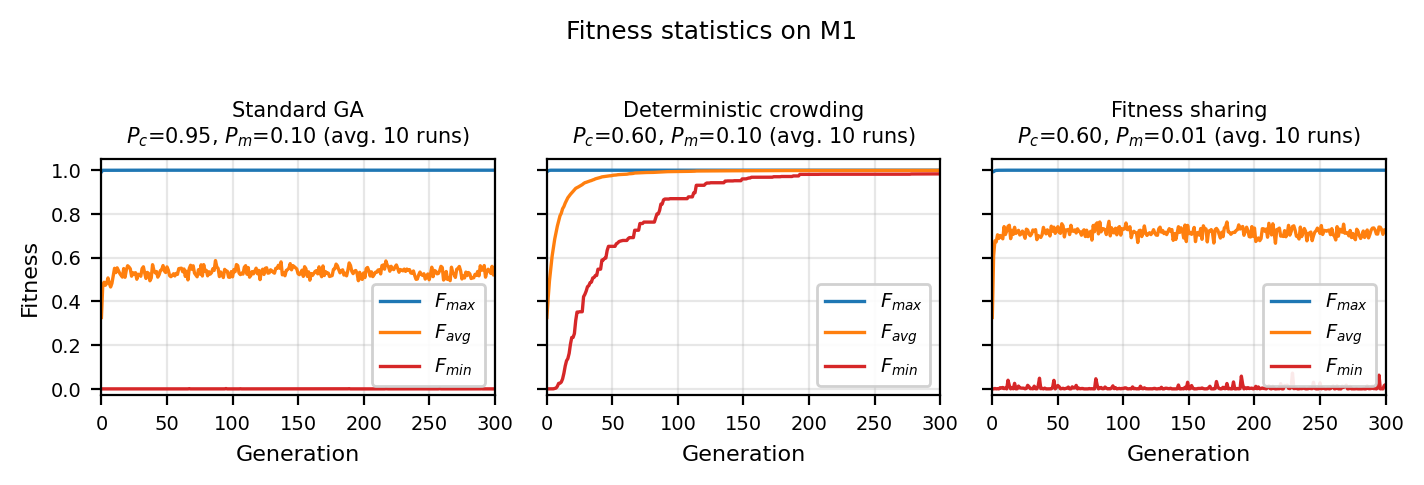
\includegraphics[width=\textwidth]{figures/fig_convergence_M1.png}
\caption{$F_{max}$, $F_{avg}$, $F_{min}$ versus generation on M1 at each
method's best configuration (average of 10 runs). Deterministic crowding
drives all three statistics to $\approx 1$: its whole population sits on the
five equal-height peaks. The standard GA's $F_{avg}$ plateaus far below the
peaks, and fitness sharing settles at an intermediate $F_{avg}$ because it
deliberately spreads individuals across niches and the slopes between them.}
\label{fig:convM1}
\end{figure*}

\begin{figure*}[t]
\centering
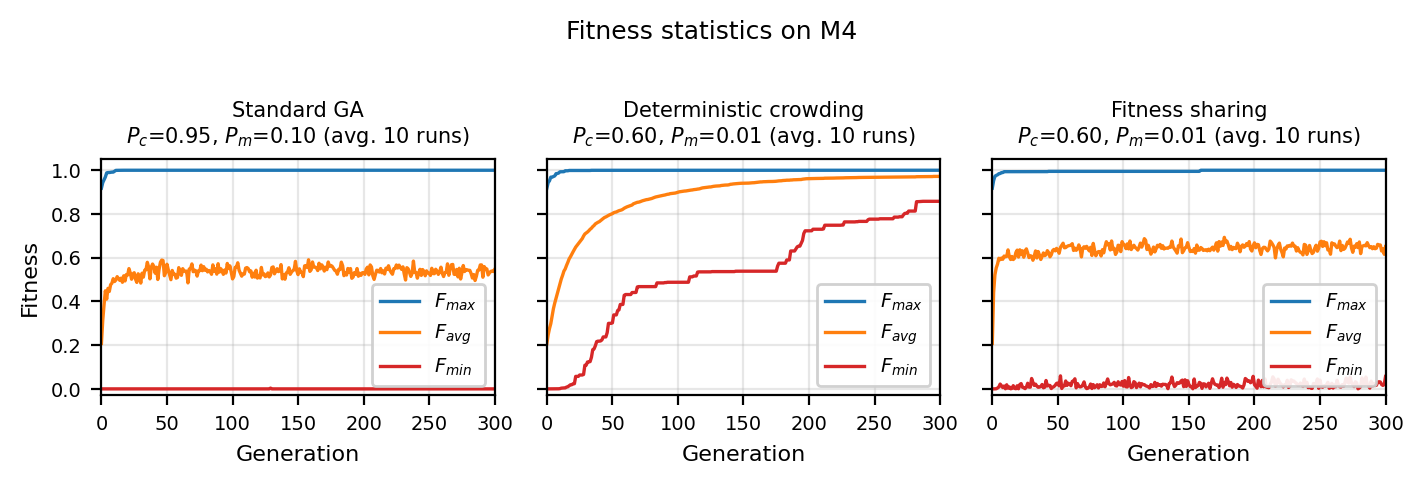
\includegraphics[width=\textwidth]{figures/fig_convergence_M4.png}
\caption{$F_{max}$, $F_{avg}$, $F_{min}$ versus generation on M4 (average of
10 runs). Crowding's $F_{min}$ climbs steadily as the population fills the
tall peaks; the standard GA and sharing keep $F_{min} \approx 0$ because
valley individuals persist. All three reach $F_{max} \approx 1$ within a few
generations.}
\label{fig:convM4}
\end{figure*}

\begin{table}[htbp]
\caption{Fitness statistics at generation 300 at each method's best
configuration (mean $\pm$ std.\ over 10 runs); Std = standard GA,
Crowd = deterministic crowding, Share = fitness sharing}
\label{tab:finalstats}
\centering
\scriptsize
\setlength{\tabcolsep}{4pt}
\begin{tabular}{@{}llccc@{}}
\toprule
Func. & Method ($P_c$/$P_m$) & $F_{max}$ & $F_{avg}$ & $F_{min}$ \\
\midrule
M1 & Std (0.95/0.10) & $1.000 \pm 0.000$ & $0.551 \pm 0.063$ & $0.000 \pm 0.000$ \\
M1 & Crowd (0.60/0.10) & $1.000 \pm 0.000$ & $0.999 \pm 0.001$ & $0.983 \pm 0.017$ \\
M1 & Share (0.60/0.01) & $1.000 \pm 0.000$ & $0.727 \pm 0.071$ & $0.019 \pm 0.061$ \\
M4 & Std (0.95/0.10) & $1.000 \pm 0.000$ & $0.547 \pm 0.042$ & $0.000 \pm 0.000$ \\
M4 & Crowd (0.60/0.01) & $1.000 \pm 0.000$ & $0.972 \pm 0.006$ & $0.858 \pm 0.142$ \\
M4 & Share (0.60/0.01) & $1.000 \pm 0.000$ & $0.651 \pm 0.054$ & $0.057 \pm 0.074$ \\
\bottomrule
\end{tabular}
\end{table}

\subsection{Peaks that survive over generations}

Figure~\ref{fig:peakstime} tracks the average number of represented peaks
versus generation. Crowding on M1 reaches all five peaks by roughly
generation 25 and holds them for the rest of the run. On M4, crowding's peak
count \emph{rises to $\approx 4.9$ by generation 25 and then decays to
$\approx 2.3$}---it explores all peaks early and later loses the short ones.
Sharing climbs to a stable plateau (M1 $\approx 4$, M4 $\approx 3.5$--$4$),
while the standard GA oscillates around 2--3 peaks and never improves.

\begin{figure*}[t]
\centering
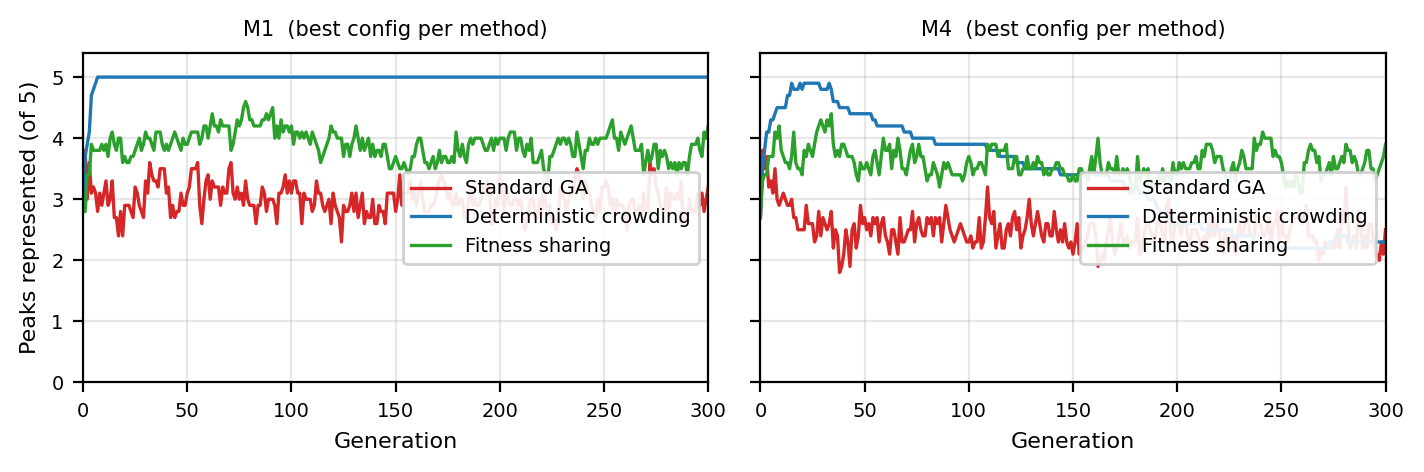
\includegraphics[width=\textwidth]{figures/fig_peaks_time.png}
\caption{Average number of the five peaks represented in the population
versus generation (best configuration per method, average of 10 runs).
Crowding is perfect on the equal-height function M1, but on M4 its peak count
collapses after an early peak as shorter niches are cannibalized; sharing is
the most stable method on M4.}
\label{fig:peakstime}
\end{figure*}

\subsection{Effect of $P_c$ and $P_m$}

Figure~\ref{fig:bars} shows the average peak count for all four
($P_c$, $P_m$) combinations. Mutation rate dominates: for the standard GA,
raising $P_m$ from 0.01 to 0.10 roughly doubles the peaks found (M1:
$1.2 \rightarrow 2.6$ at $P_c=0.60$; $1.1 \rightarrow 3.2$ at $P_c=0.95$),
because mutation is the only remaining source of diversity once selection
concentrates the population. Crowding is insensitive to both rates on M1
($5.0$ everywhere) and mildly sensitive on M4 (best at low $P_c$ and low
$P_m$). Sharing degrades slightly at high $P_c$ on M1
($4.2 \rightarrow 3.8$ at $P_m=0.01$) but is otherwise flat. Crossover rate
has a much smaller effect than mutation rate for every method.

\begin{figure*}[t]
\centering
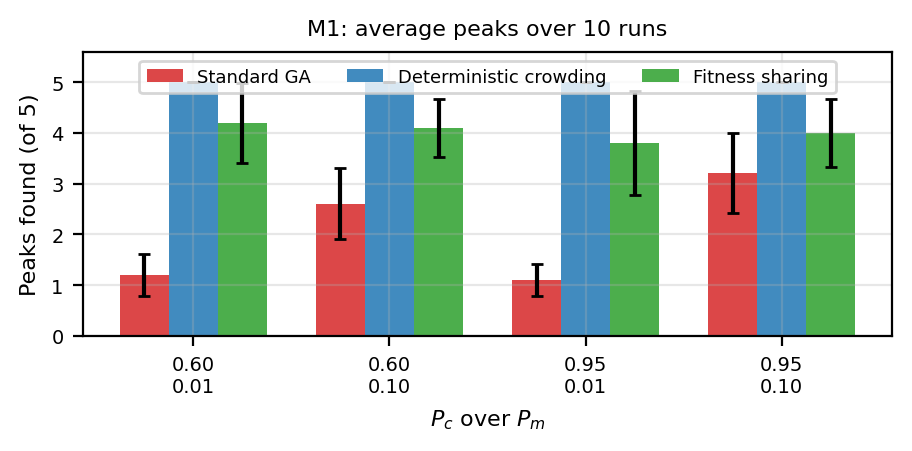
\includegraphics[width=0.49\textwidth]{figures/fig_peaks_bars_M1.png}
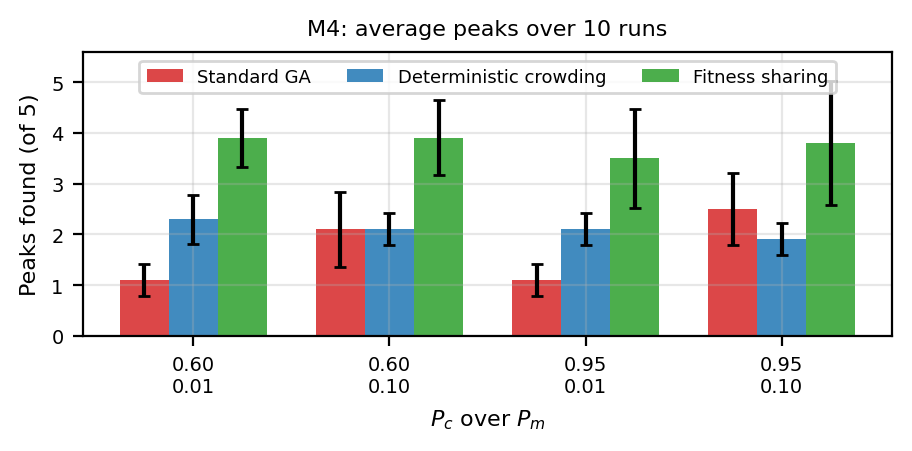
\includegraphics[width=0.49\textwidth]{figures/fig_peaks_bars_M4.png}
\caption{Average peaks found (of 5) over 10 runs for every
($P_c$, $P_m$) configuration; error bars are one sample standard deviation.
Left: M1. Right: M4.}
\label{fig:bars}
\end{figure*}

\subsection{Population on the landscape}

Figures~\ref{fig:landM1} and~\ref{fig:landM4} show the initial and final
populations of the best run of the best configuration for each method, over
the fitness landscape.

\begin{figure*}[t]
\centering
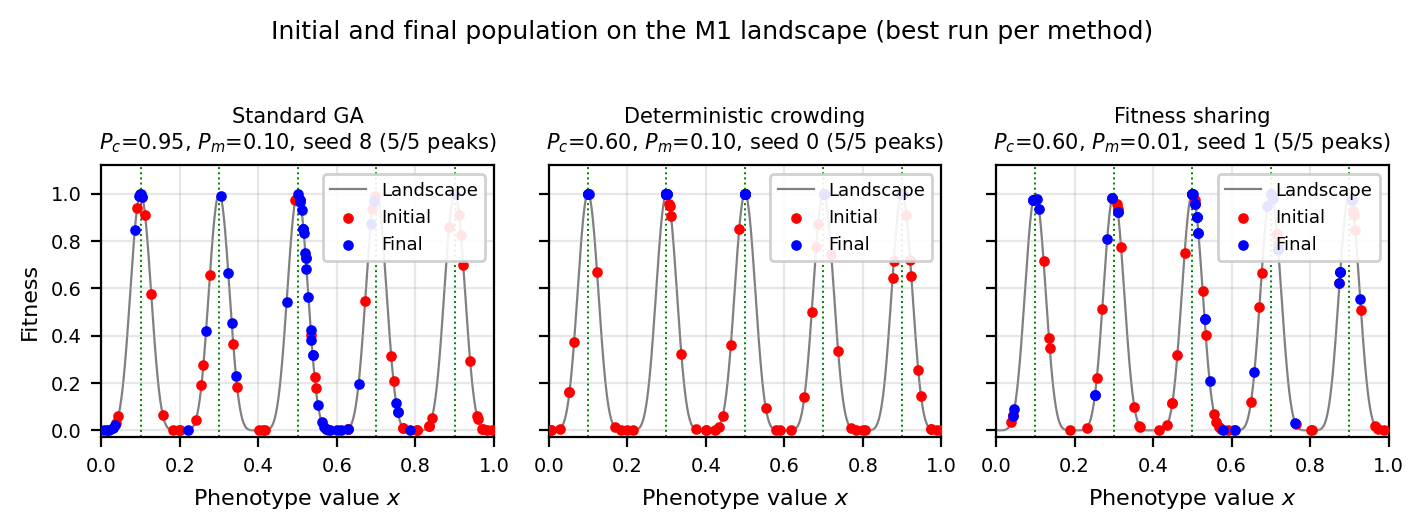
\includegraphics[width=\textwidth]{figures/fig_landscape_M1.png}
\caption{Initial (red) and final (blue) population over the M1 landscape for
the best run of each method's best configuration. The standard GA's final
population clusters on a few peaks with many individuals stranded in the
valleys; crowding's population occupies all five peaks; sharing spreads
individuals across every peak and its slopes.}
\label{fig:landM1}
\end{figure*}

\begin{figure*}[t]
\centering
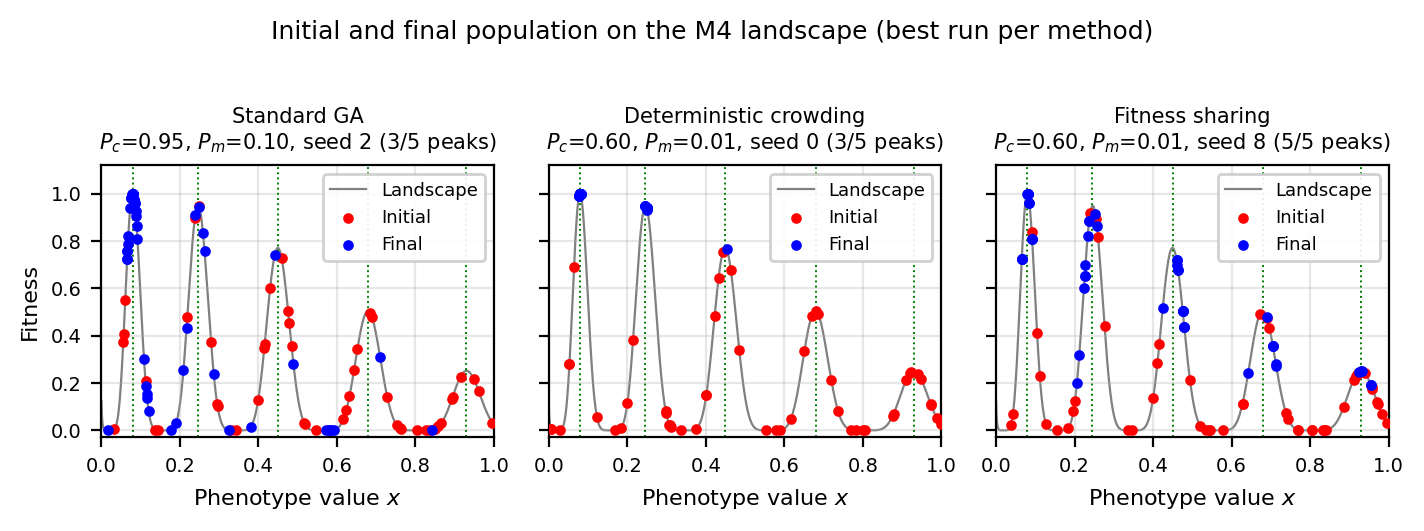
\includegraphics[width=\textwidth]{figures/fig_landscape_M4.png}
\caption{Initial (red) and final (blue) population over the M4 landscape.
Sharing is the only method whose best run occupies all five peaks; crowding's
population concentrates on the two tallest peaks, and the standard GA covers
only the tallest peak densely.}
\label{fig:landM4}
\end{figure*}

\section{Analysis of Results}
\label{sec:analysis}

\textbf{Why crowding wins M1 but loses M4.} Deterministic crowding replaces a
parent only when the child is \emph{strictly fitter}. On M1 all five peaks
have equal height ($f=1$), so a child that migrates onto another equal-height
peak is never strictly fitter than the resident and cannot evict it; each
occupied peak is therefore stable, and crowding attains $5.0 \pm 0.00$ in all
four configurations with $F_{avg} = 0.999$ and $F_{min} = 0.983$---the entire
population lives on peaks. On M4 the peaks are unequal
($1.00, 0.95, 0.77, 0.50, 0.25$). A child born near a \emph{tall} peak and
matched to the \emph{short}-peak parent by Hamming distance \emph{is} strictly
fitter than that parent, so it replaces it; over generations, individuals leak
from the short peaks into the tall ones. The per-peak hit rates confirm the
mechanism: at its best configuration, crowding found the M4 peaks at
$x=0.08$ and $0.245$ in 10/10 runs, but $x=0.45$ in only 2/10, $x=0.68$ in
1/10, and $x=0.93$ in 0/10. The peak-survival plot (M4 panel of
Fig.~\ref{fig:peakstime}) shows the same story in time: $\approx 4.9$ peaks at
generation 25 decaying to $\approx 2.3$ at generation 300. The strict
improvement test that makes crowding perfectly stable on equal peaks is
exactly what makes it unstable on unequal ones.

\textbf{Why sharing is the most robust method.} Sharing has no such
height-dependence: a crowded niche is penalized regardless of how tall its
peak is, so selection pressure is redirected toward whichever peaks are
under-occupied, no matter how short. This is why sharing is the only method
whose best M4 run occupies all five peaks (hit rates 10/10, 10/10, 10/10,
7/10, 2/10) and why it is the most stable method on M4
($3.5$--$3.9$ peaks, plateau reached and held). The cost of sharing is
visible in Table~\ref{tab:finalstats}: its $F_{avg}$ (0.65--0.73) is much
lower than crowding's (0.97--1.00), because individuals are intentionally
kept on the slopes and in the smaller niches rather than packed onto the
tallest peaks. Low $F_{avg}$ here is the \emph{price of diversity}, not a
failure.

\textbf{Why the standard GA fails.} Without a niching mechanism, roulette
selection amplifies whichever peak is currently ahead and genetic drift
removes the rest. Its peak count never exceeds $3.2$ on M1 or $2.5$ on M4,
and at $P_m=0.01$ it collapses to $\approx 1.1$ peaks on both functions.
Its high $F_{avg}$ at low mutation (0.946 on M1 at $P_c/P_m=0.60/0.01$,
Table~\ref{tab:peaks} context) is a symptom of that collapse---the
population has converged onto one peak, so the mean fitness is high while
diversity is gone. This is the clearest demonstration that $F_{max}$ and
$F_{avg}$ alone mislead: the configuration with the \emph{highest} average
fitness is among the \emph{worst} at peak discovery.

\textbf{Effect of the genetic operators.} Mutation rate is the main diversity
knob for the standard GA ($+1.0$ to $+2.1$ peaks going from $P_m=0.01$ to
$0.10$), while both niching methods are far less sensitive to it, because
their replacement rules---not the mutation rate---control diversity. Crossover
rate matters little: higher $P_c$ helps the standard GA slightly on M1 at
high $P_m$ ($2.6 \rightarrow 3.2$) but hurts sharing slightly
($4.2 \rightarrow 3.8$), and crowding is unchanged. Overall, the choice of
\emph{method} dominates the choice of parameters: the worst niching
configuration outperforms the best standard-GA configuration on M1
($3.8$ vs.\ $3.2$) and on M4 ($3.5$ vs.\ $2.5$).

\textbf{Landscape confirmation.} The landscape plots agree with the
statistics: on M1, crowding's final population sits on all five peaks while
the standard GA leaves individuals stranded in valleys
(Fig.~\ref{fig:landM1}); on M4, only sharing's best run covers all five
peaks, with crowding concentrated on the two tallest
(Fig.~\ref{fig:landM4}).

\section{Conclusions}
\label{sec:conclusions}

Both niching methods substantially outperform the standard GA on the
multimodal benchmarks M1 and M4: the best standard-GA configuration finds
$3.2$ of 5 peaks on M1 and $2.5$ on M4, versus $5.0$ (crowding, M1) and
$3.9$ (sharing, M4) for the niching methods. The two niching methods have
complementary strengths: deterministic crowding is perfect when peaks have
equal height but systematically cannibalizes shorter peaks when they do not,
while fitness sharing is the most robust method across both landscapes,
trading some average fitness for stable multi-peak coverage.

What we learned: (i) best fitness ($F_{max}$) saturates on these benchmarks
and must be supplemented with diversity measures such as peak counts and
$F_{min}$; (ii) a niching method's replacement rule encodes an assumption
about the landscape---crowding assumes comparable peak heights---and that
assumption should be checked against the problem; (iii) mutation rate
controls diversity only when the replacement rule does not.

Possible improvements: adaptive or per-niche $\sigma$ for sharing (a fixed
$\sigma=0.10$ cannot serve peaks of very different widths), a crowding
variant with a distance- and height-aware acceptance test (e.g., restricted
tournament selection), a larger population to give each of the five niches
more room, and extension to the remaining benchmark functions M2, M3, and M5+
to test whether the observed ranking generalizes.

\begin{thebibliography}{9}
\bibitem{b1} D. E. Goldberg, \emph{Genetic Algorithms in Search,
Optimization and Machine Learning}. Addison-Wesley, 1989.
\bibitem{b2} S. W. Mahfoud, ``A comparison of parallel and sequential
niching methods,'' in \emph{Proc. 6th Int. Conf. on Genetic Algorithms
(ICGA)}, 1995, pp. 136--143.
\bibitem{b3} D. E. Goldberg and J. Richardson, ``Genetic algorithms with
sharing for multimodal function optimization,'' in \emph{Proc. 2nd Int.
Conf. on Genetic Algorithms (ICGA)}, 1987, pp. 41--49.
\bibitem{b4} K. Spurlock and M. Fukuyama, ``Niching GA example,''
\texttt{niching\_ga\_examplever.py}, CSE 620 course notebook, 2022.
\end{thebibliography}

\appendices

\section{Demo Video}
\label{app:video}

A $\sim$5-minute screen recording walking through the code, the experimental
methodology, the findings, and the most challenging/rewarding aspects of the
project. Replace the placeholder below with your SharePoint / Google Drive /
YouTube (unlisted) link before submitting:

\url{[VIDEO-LINK-PLACEHOLDER]}

\section{Additional Figures}
\label{app:figs}

\begin{figure*}[htbp]
\centering
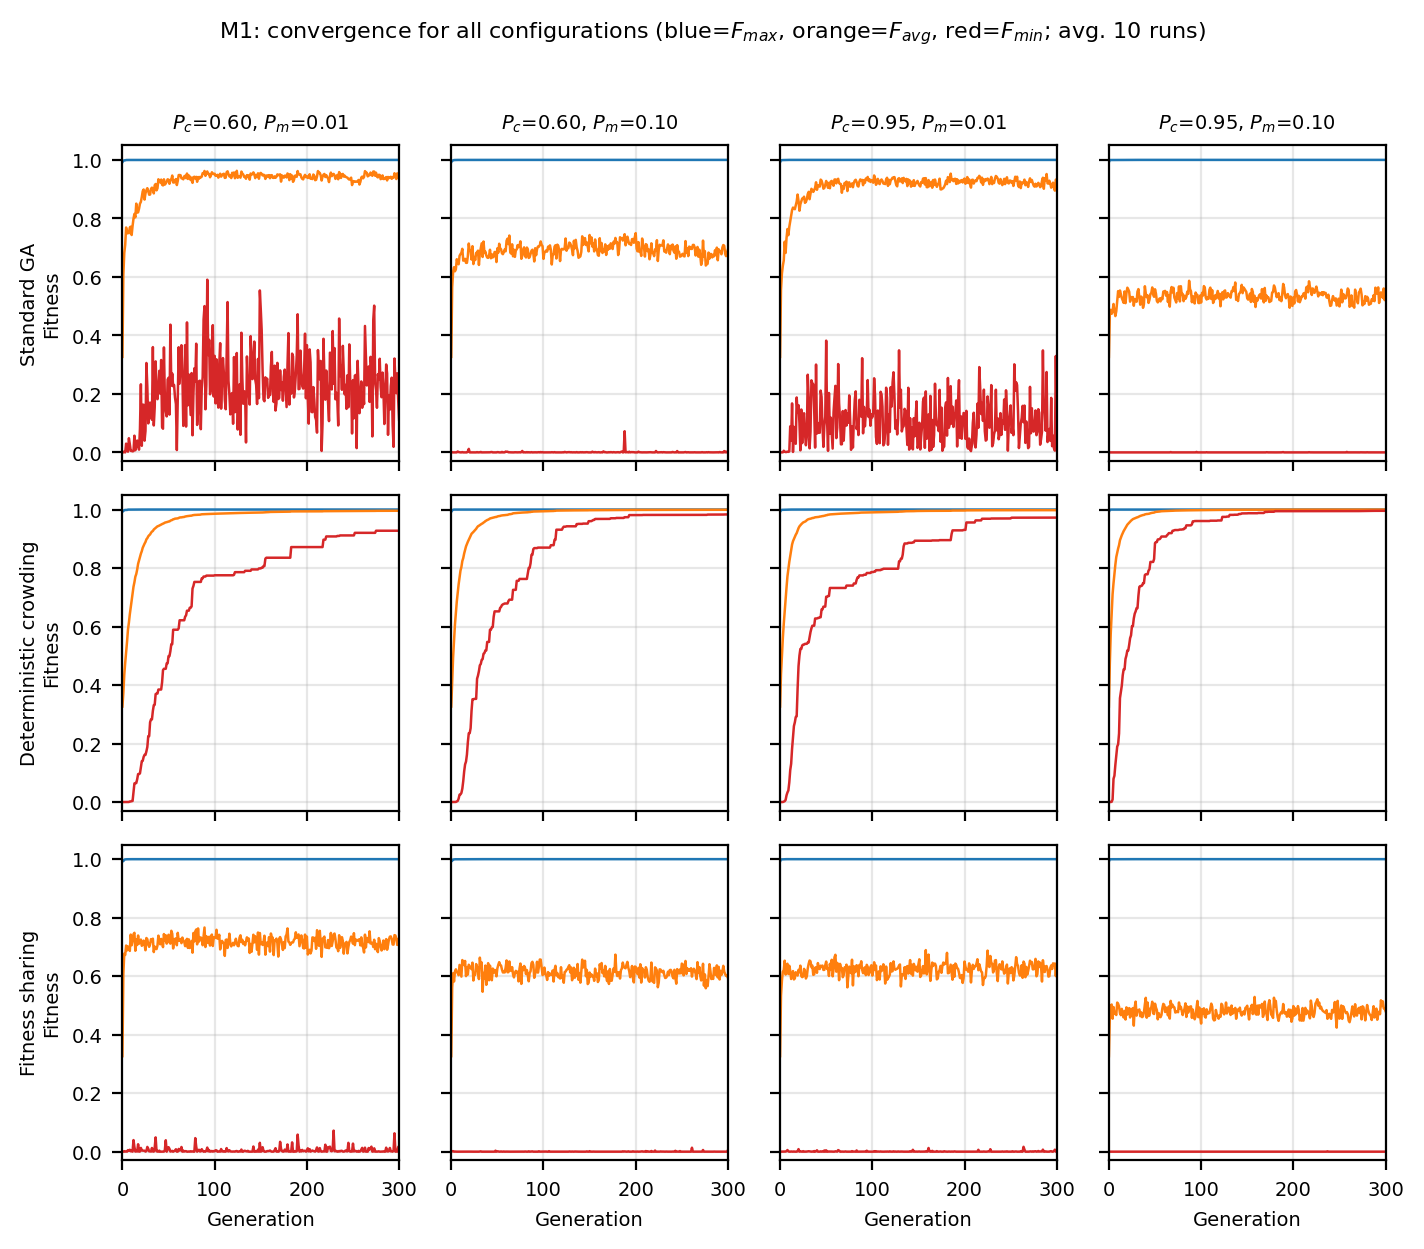
\includegraphics[width=\textwidth]{figures/fig_conv_grid_M1.png}
\caption{Appendix: $F_{max}$/$F_{avg}$/$F_{min}$ versus generation for every
(method, $P_c$, $P_m$) configuration on M1 (average of 10 runs).}
\label{fig:gridM1}
\end{figure*}

\begin{figure*}[htbp]
\centering
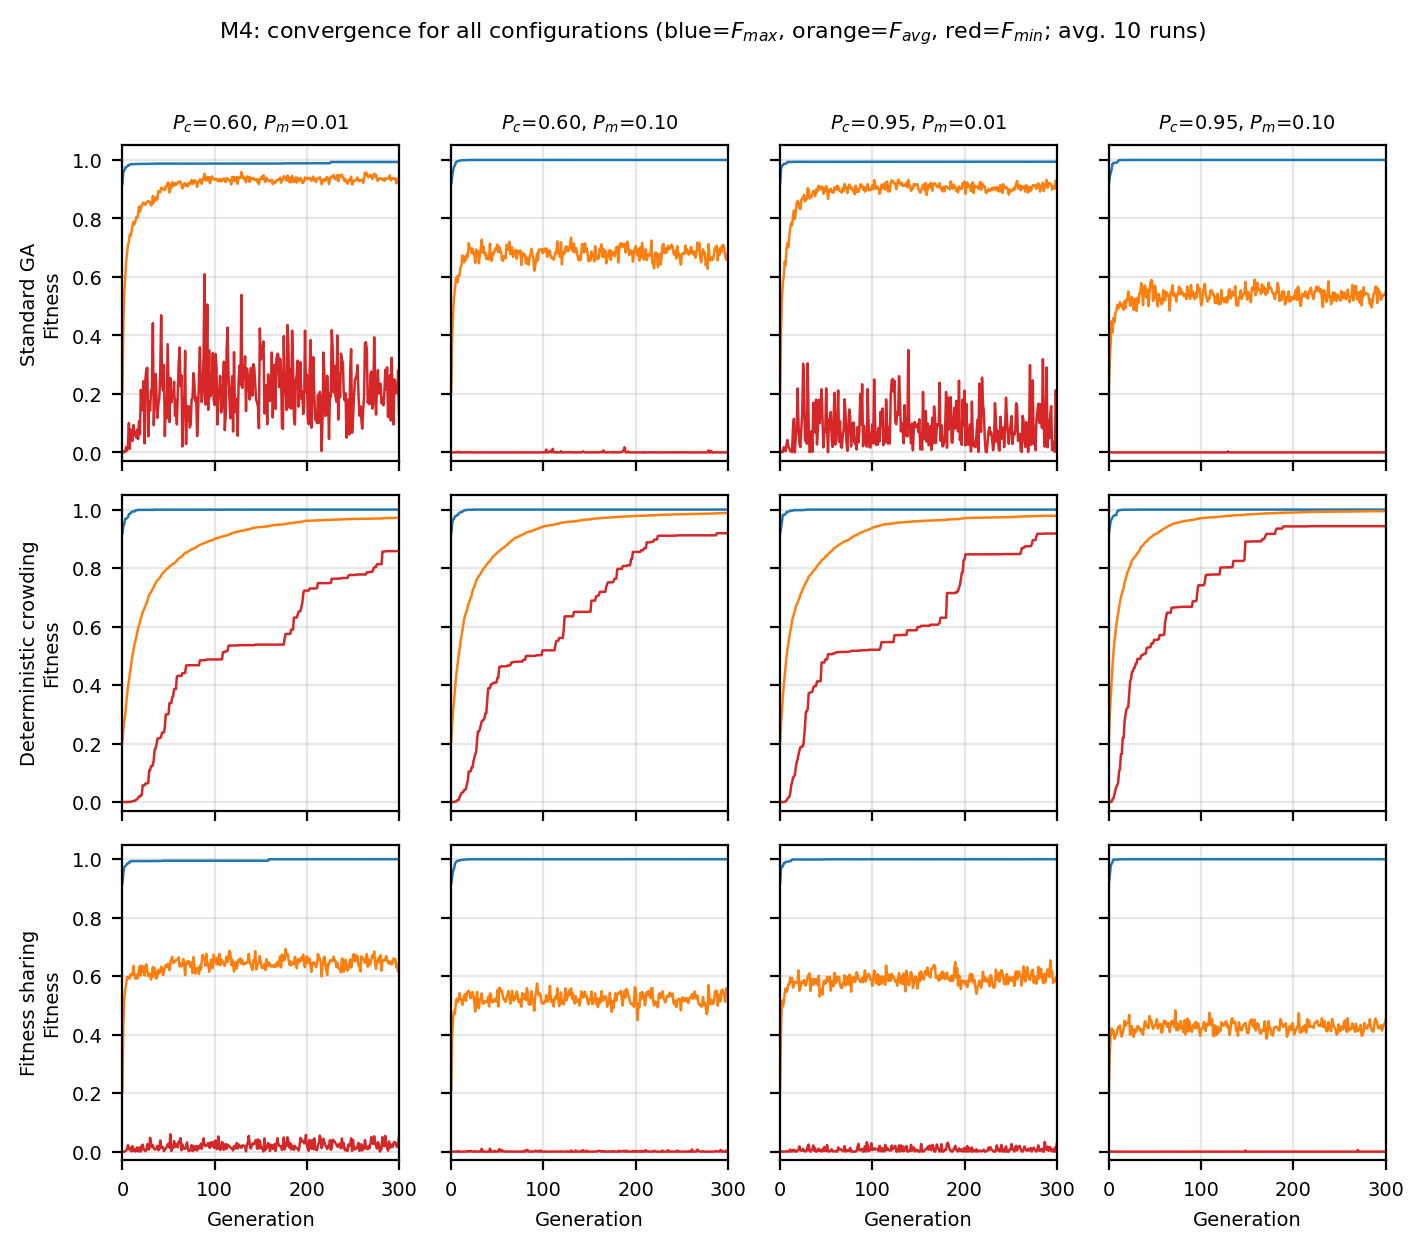
\includegraphics[width=\textwidth]{figures/fig_conv_grid_M4.png}
\caption{Appendix: $F_{max}$/$F_{avg}$/$F_{min}$ versus generation for every
(method, $P_c$, $P_m$) configuration on M4 (average of 10 runs).}
\label{fig:gridM4}
\end{figure*}

\end{document}
